\documentclass{article}
\usepackage{amsmath}
\usepackage{amssymb}
\usepackage{graphicx}
\usepackage{hyperref}
\usepackage[version=4]{mhchem}

\title{Example 1}
\date{}

\begin{document}
\maketitle

In triangle \(A B C, \angle C=90^{\circ} . \angle 1=\angle 2 . C D=15 \mathrm{~mm}, B D=25 \mathrm{~mm}\). Find \(A C\).

Solution: 30 mm .\\
Draw \(D E \perp A B\) so that the perpendicular line meets \(A B\) at \(E . \triangle C A D\) and \(\triangle A E D\) are congruent and \(D E=C D=\)\\
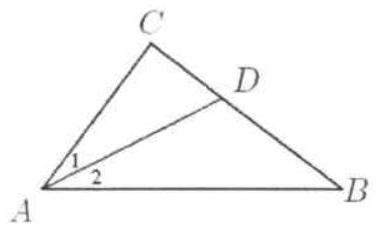
\includegraphics[width=\textwidth]{images/problem_image_1.jpg} \(15 \mathrm{~mm} . \triangle D B E\) is a \(15-20-25\) right triangle and is similar to \(\triangle A B C\).

\[
\frac{A C}{C B}=\frac{D E}{E B} \Rightarrow \frac{A C}{15+25}=\frac{15}{25} \Rightarrow \quad A C=30
\]

\begin{center}
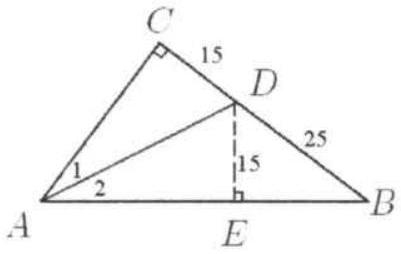
\includegraphics[width=\textwidth]{images/reasoning_image_1.jpg}
\end{center}


\end{document}
